% ------------------------------------------------------------------------------
% Chapter 1
% Delete this content and replace with your own
% ------------------------------------------------------------------------------
\chapter{Methodology} % enter the name of the chapter here
\label{cha:chapter label} % enter the chapter label here (for cross referencing)
We used a bunch of functions and methods to make the project a succesful one. In this chapter we will be discusing about those functions and methos.

\section{Detecting Fingers} % enter the name of the section here
\label{sec:section label} % enter the section label here (for cross referencing)
The function, \texttt{NoOfFingers()}, captures video from the default camera (0) and detects hands in the video using an instance of the \texttt{HandDetector} class. The \texttt{HandDetector} class is responsible for detecting hands in an image using computer vision techniques. The function reads a single frame of video using \texttt{cv2.VideoCapture} and passes it to the \texttt{HandDetector} instance's \texttt{findHands} method, which returns an image with the detected hands and a list of hand regions in the image. The function then counts the number of fingers raised in the first hand detected using the \texttt{fingersUp} method. Finally, the function returns the number of fingers and the number of hands detected as a tuple. If no hands are detected, the function returns (0, 0).


 \section{The Main Game Loop} % enter the name of the section here
\label{sec:section label}
In the main game loop, the \texttt{slideTo} variable will track which direction the player wants to slide a tile (it starts off at the beginning of the game loop as None and is set later) and the \texttt{msg} variable tracks what string to display at the top of the window. The program does a quick check if the board data structure has the same value as the solved board data structure stored in \texttt{SOLVEDBOARD}. If so, then the \texttt{msg} variable is changed to the string 'Solved!'.
This won’t appear on the screen until \texttt{drawBoard()} has been called to draw it to the \texttt{DISPLAYSURF} Surface object and \texttt{pygame.display.update()} is called to draw the display Surface object on the actual computer screen.

\subsection{Handling Events} % enter the name of the section here
\label{sec:section label}
Before going into the event loop, the program calls \texttt{checkForQuit()} to see if any QUIT events have been created (and terminates the program if there have). Why we have a separate function (the \texttt{checkForQuit()} function) for handling the QUIT events will be explained later. The for loop executes the event handling code for any other event created since the last time \texttt{pygame.event.get()} was called (or since the program started, if \texttt{pygame.event.get()} has never been called before).
If the type of event was a \texttt{MOUSEBUTTONUP} event (that is, the player had released a mouse button somewhere over the window), then we pass the mouse coordinates to our \texttt{getSpotClicked()} function which will return the board coordinates of the spot on the board the mouse release happened. The \texttt{event.pos[0]} is the X coordinate and \texttt{event.pos[1]} is the Y coordinate.
If the mouse button release did not happen over one of the spaces on the board (but obviously still happened somewhere on the window, since a \texttt{MOUSEBUTTONUP} event was created), then \texttt{getSpotClicked()} will return None. If this is the case, we want to do an additional check to see if the player might have clicked on the Reset, New, or Solve buttons (which are not located on the board).

The coordinates of where these buttons are on the window are stored in the \texttt{pygame.Rect} objects. We can pass the mouse coordinates from the Event object to the \texttt{collidepoint()} method. This method will return True if the mouse coordinates are within the \texttt{Rect} object’s area and False otherwise.

\subsubsection{Checking QUIT Events} %enter the name of the subsection here
\label{sec:subsection label} % enter the subsection label here (for cross referencing)
The \texttt{checkForQuit()} function will check for QUIT events (or if the user has pressed the \texttt{Esc} key) and then call the \texttt{terminate()} function. But this is a bit tricky and requires some explanation.
PyGame internally has its own list data structure that it creates and appends Event objects to as they are made. This data structure is called the event queue. When the \texttt{pygame.event.get()} function is called with no parameters, the entire list is returned. However, you can pass a constant like \texttt{QUIT} to \texttt{pygame.event.get()} so that it will only return the \texttt{QUIT} events (if any) that are in the internal event queue. The rest of the events will stay in the event queue for the next time \texttt{pygame.event.get()} is called.

\subsubsection{Sliding Tiles with the Mouse} %enter the name of the subsection here
\label{sec:subsection label} % enter the subsection label here (for cross referencing)
If \texttt{getSpotClicked()} did not return (None, None), then it will have returned a tuple of two integer values that represent the X and Y coordinate of the spot on the board that was clicked. Then the if and \texttt{elif} statements check if the spot that was clicked is a tile that is next to the blank spot (otherwise the tile will have no place to slide).
Our \texttt{getBlankPosition()} function will take the board data structure and return the X and Y board coordinates of the blank spot, which we store in the variables \texttt{blankx} and \texttt{blanky}. If the spot the user clicked on was next to the blank space, we set the \texttt{slideTo} variable with the value that the tile should slide.

\subsubsection{Sliding Tiles with the Keyboard} %enter the name of the subsection here
\label{sec:subsection label} % enter the subsection label here (for cross referencing)
We can also let the user slide tiles by pressing keyboard keys. The \texttt{if} and \texttt{elif} statements let the user set the \texttt{slideTo} variable by either pressing the arrow keys or the WASD keys (explained later). Each \texttt{if} and \texttt{elif} statement also has a call to v{isValidMove()} to make sure that the tile can slide in that direction. (We didn’t have to make this call with the mouse clicks because the checks for the neighboring blank space did the same thing.)
\subsubsection{Sliding Tiles with Hand Gestures} %enter the name of the subsection here
\label{sec:subsection label} % enter the subsection label here (for cross referencing)
After the event loop is finished the program checks whether the game mode is now \texttt{HAND} mode. If so then \texttt{FingerDetector.NoOfFingers()} is called and number of fingers, hands are calculated. If the hands is not zero then the program checks appropriate number of fingers for appropriate move. If the \texttt{fingers == 1} then \texttt{slideTo = UP}, \texttt{if fingers == 2} then \texttt{slideTo = DOWN}, \texttt{if fingers == 3} then \texttt{slideTo = RIGHT, if fingers == 4} then \texttt{slideTo = LEFT}  is assigned and also checks whether the move is valid or not by calling \texttt{isValidMove(mainBoard, MOVE)} function which checks whether the move position is blank or not. If it is blank then the move is valid and \texttt{isValidMove(mainBoard, MOVE)} returns \texttt{True} otherwise returns \texttt{False}.
\section{Creating the Board Data Structure} %enter the name of the subsection here
\label{sec:subsection label} % enter the subsection label here (for cross referencing)
The \texttt{getStartingBoard()} data structure will create and return a data structure that represents a ―solved board, where all the numbered tiles are in order and the blank tile is in the lower right corner. This is done with nested for loops, just like the board data structure in the Memory Puzzle game was made.
However, notice that the first column isn’t going to be [1, 2, 3] but instead [1, 4, 7]. This is because the numbers on the tiles increase by 1 going across the row, not down the column. Going down the column, the numbers increase by the size of the board’s width (which is stored in the \texttt{BOARDWIDTH} constant). We will use the counter variable to keep track of the number that should go on the next tile. When the numbering of the tiles in the column is finished, then we need to set counter to the number at the start of the next column.
\subsection{Drawing the board} %enter the name of the subsection here
\label{sec:subsection label} % enter the subsection label here (for cross referencing)
This function handles drawing the entire board and all of its tiles to the \texttt{DISPLAYSURF} display Surface object. The fill() method completely paints over anything that used to be drawn on the display Surface object before so that we start from scratch.
Then the program handles drawing the message at the top of the window. We use this for the ―"Generating new puzzle..." and other text we want to display at the top of the window. Remember that if statement conditions consider the blank string to be a False value, so if message is set to '' then the condition is False.
Next, nested for loops are used to draw each tile to the display Surface object by calling the \texttt{drawTile()} function.
\subsubsection{Drawing a Tile} %enter the name of the subsection here
\label{sec:subsection label} % enter the subsection label here (for cross referencing)
The \texttt{drawTile()} function will draw a single numbered tile on the board. The \texttt{tilex} and \texttt{tiley} parameters are the board coordinates of the tile. The number parameter is a string of the tile’s number (like '3' or '12'). The \texttt{adjx} and \texttt{adjy} keyword parameters are for making minor adjustments to the position of the tile. For example, passing 5 for \texttt{adjx} would make the tile appear 5 pixels to the right of the \texttt{tilex} and \texttt{tiley} space on the board. Passing -10 for \texttt{adjx} would make the tile appear 10 pixels to the left of the space.
These adjustment values will be handy when we need to draw the tile in the middle of sliding. If no values are passed for these arguments when \texttt{drawTile()} is called, then by default they are set to 0. This means they will be exactly on the board space given by \texttt{tilex} and \texttt{tiley}.
The PyGame drawing functions only use pixel coordinates, this program converts the board coordinates in \texttt{tilex} and \texttt{tiley} to pixel coordinates, which we will store in variables left and top (since \texttt{getLeftTopOfTile()} returns the top left corner’s coordinates). We draw the background square of the tile with a call to \texttt{pygame.draw.rect()} while adding the \texttt{adjx} and \texttt{adjy} values to left and top in case the code needs to adjust the position of the tile.
Then creating the Surface object that has the number text drawn on it. A \texttt{Rect} object for the Surface object is positioned, and then used to \texttt{blit} the Surface object to the display Surface. The \texttt{drawTile()} function doesn’t call \texttt{pygame.display.update()} function, since the caller of \texttt{drawTile()} probably will want to draw more tiles for the rest of the board before making them appear on the screen.
\subsubsection{Making Text Appear on the Screen} %enter the name of the subsection here
\label{sec:subsection label} % enter the subsection label here (for cross referencing)
The \texttt{makeText()} function handles creating the Surface and \texttt{Rect} objects for positioning text on the screen. Instead of doing all these calls each time we want to make text on the screen, we can just call \texttt{makeText()} instead. This saves us on the amount of typing we have to do for our program. (Though \texttt{drawTile()} makes the calls to render() and $get_rect()$ itself because it positions the text Surface object by the center point rather than the \texttt{topleft} point and uses a transparent background color.)
\subsection{Creating a New Puzzle}
The \texttt{generateNewPuzzle()} function will be called at the start of each new game. It will create a new board data structure by calling \texttt{getStartingBoard()} and then randomly scramble it. The first few lines of \texttt{generateNewPuzzle() }get the board and then draw it to the screen (freezing for half a second to let the player see the fresh board for a moment).
The \texttt{numSlides} parameter will show tell the function how many of these random moves to make. The code for doing a random move is the \texttt{getRandomMove()} call to get the move itself, then call \texttt{slideAnimation()} to perform the animation on the screen. Because doing the slide animation does not actually update the board data structure, we update the board by calling \texttt{makeMove()}.
We need to keep track of each of the random moves that was made so that the player can click the ―Solve button later and have the program undo all these random moves. So the move is appended to the list of moves in sequence.
Then we store the random move in a variable called \texttt{lastMove} which will be passed to \texttt{getRandomMove()} on the next iteration. This prevents the next random move from undoing the random move we just performed.
All of this needs to happen \texttt{numSlides} number of times, so we put \texttt{getRandomMove()} inside a for loop. When the board is done being scrambled, then we return the board data structure and also the list of the random moves made on it.
\subsubsection{Animating the Tile Slides}
The first thing our tile sliding animation code needs to calculate is where the blank space is and where the moving tile is. The code that calls \texttt{slideAnimation()} should make sure that the slide it passes for the direction parameter is a valid move to make.
In order to draw the frames of the sliding animation, we must draw the \texttt{baseSurf} surface on the display Surface, then on each frame of the animation draw the sliding tile closer and closer to its final position where the original blank space was. The space between two adjacent tiles is the same size as a single tile, which we have stored in \texttt{TILESIZE}. The code uses a for loop to go from 0 to \texttt{TILESIZE}.
Normally this would mean that we would draw the tile 0 pixels over, then on the next frame draw the tile 1 pixel over, then 2 pixels, then 3, and so on. Each of these frames would take \texttt{1/30th} of a second. If you have \texttt{TILESIZE} set to 80 (as the program in this book does on line 12) then sliding a tile would take over two and a half seconds, which is actually kind of slow.
So instead we will have the for loop iterate from 0 to \texttt{TILESIZE} by several pixels each frame. The number of pixels it jumps over is stored in \texttt{animationSpeed}, which is passed in when \texttt{slideAnimation()} is called. For example, if \texttt{animationSpeed} was set to 8 and the constant \texttt{TILESIZE} was set to 80, then the for loop and \texttt{range(0, TILESIZE, animationSpeed)} would set the i variable to the values 0, 8, 16, 24, 32, 40, 48, 56, 64, 72. (It does not include 80 because the range() function goes up to, but not including, the second argument.) This means the entire sliding animation would be done in 10 frames, which would mean it is done in \texttt{10/30th} of a second (a third of a second) since the game runs at 30 FPS.
\subsubsection{Getting Random Moves}
At the beginning of the game, we start with the board data structure in the solved, ordered state and create the puzzle by randomly sliding around tiles. To decide which of the four directions we should slide, we’ll call our \texttt{getRandomMove()} function. Normally we could just use the random.choice() function and pass it a tuple (UP, DOWN, LEFT, RIGHT) to have Python simply randomly choose a direction value for us. But the Sliding Puzzle game has a small restriction that prevents us from choosing a purely random number.
If you had a slide puzzle and slid a tile to left, and then slid a tile to the right, you would end up with the exact same board you had at the start. It’s pointless to make a slide followed by the opposite slide. Also, if the blank space is in the lower right corner than it is impossible to slide a tile up or to the left.
The code in \texttt{getRandomMove()} will take these factors into account. To prevent the function from selecting the last move that was made, the caller of the function can pass a directional value for the \texttt{lastMove} parameter. Then wetake a list of all four directional values stored in the \texttt{validMoves} variable. The \texttt{lastMove} value (if not set to None) is removed from \texttt{validMoves}. Depending on if the blank space is at the edge of the board,then we remove other directional values from the \texttt{lastMove} list.
Of the values that are left in \texttt{lastMove}, one of them is randomly selected with a call to random.choice() and returned.
\subsection{Animating the Board on "Reset" or "Solve"}
When the player clicks on ―Reset or ―Solve, the Slide Puzzle game program needs to undo all of the moves that were made to the board. The list of directional values for the slides will be passed as the argument for the \texttt{allMoves} parameter.
We use list slicing to create a duplicate of the \texttt{allMoves} list. Remember that if you don’t specify a number before the :, then Python assumes the slice should start from the very beginning of the list. And if you don’t specify a number after the :, then Python assumes the slice should keep going to the very end of the list. So \texttt{allMoves[:]} creates a list slice of the entire \texttt{allMoves} list. This makes a copy of the actual list to store in \texttt{revAllMoves}, rather than just a copy of the list reference.
To undo all the moves in \texttt{allMoves}, we need to perform the opposite move of the moves in \texttt{allMoves}, and in reverse order. There is a list method called reverse() which will reverse the order of the items in a list. We call this on the \texttt{revAllMoves} list on line 316.
Then a for loop iterates over the list of directional values. Then we call \texttt{slideAnimation()} to perform the animation, and \texttt{makeMove()} to update the board data structure.
\section{The Auto Solve Algorithm}
Solving a slide puzzle can be really tricky. We could program the computer to do it, but that would require us to figure out an algorithm that can solve the slide puzzle. That would be very difficult and involve a lot of cleverness and effort to put into this program.
Fortunately, there’s an easier way. We could just have the computer memorize all the random slides it made when it created the board data structure, and then the board can be solved just by performing the opposite slide. Since the board originally started in the solved state, undoing all the slides would return it to the solved state.
Suppose, after the right slide, if we do the opposite slide (a left slide) then the board will be back in the original state. So to get back to the original state after several slides, we just have to do the opposite slides in reverse order. If we did a right slide, then another right slide, then a down slide, we would have to do an up slide, left slide, and left slide to undo those first three slides. This is much easier than writing a function that can solve these puzzles simply by looking at the current state of them.
% \blindtext[1]
% \subsection{Some maths}

% % ------------------------------------------------------------------------------
% % Math mode examples
% % ------------------------------------------------------------------------------

% \LaTeX\ is very good at presenting mathematics.

% Inline equation :
% $ax^2 + bx + c = 0$ % note use of single $ signs

% Display equation:
% $$x = \frac{-b \pm \sqrt{b^2 - 4ac}}{2a}$$ % note use of double $$ signs

% Numbered equation:
% \begin{align}
% 	\label{eq:equation label} % enter the equation label here (for cross referencing)
% 	\frac{\partial}{\partial t} U + \nabla \cdot F = 0
% \end{align}

% Aligned equation (not how equals signs line up):
% \begin{align}
% 	\notag % means the current line will not be numbered
% 	\label{eq:dot product}
% 	\textbf{a} \cdot \textbf{b} &= \sum_{i=1}^n a_ib_i \\
% 	&= a_1b_1 + a_2b_2 + \cdots + a_nb_n; % the & is used as the alignment guide
% \end{align}

% Aligned equation with no numbers:
% \begin{align*} % note use of *
% 	\label{eq:dot product}
% 	\textbf{a} \cdot \textbf{b} &= \sum_{i=1}^n a_ib_i \\
% 	&= a_1b_1 + a_2b_2 + \cdots + a_nb_n;
% \end{align*}

% \subsection{Theorems, proofs, definitions and examples}

% % ------------------------------------------------------------------------------
% % Theorems, proofs, definitions and examples
% % ------------------------------------------------------------------------------
% \begin{theorem}[Fermat's last theorem]
% No three positive integers $a$, $b$, and $c$ satisfy the equation $a^n + b^n = c^n$ for any integer value of n greater than 2.
% \end{theorem}

% \begin{proof}
% Left as an exercise for the reader.
% \end{proof}

% \begin{definition}
% The intersection of two sets $A$ and $B$, denoted by $A \cap B$, is the set of all objects that are members of both the sets $A$ and $B$.
% \end{definition}

% \begin{example}
% Given the two sets $A = \{x:x\in \mathbb{N}, x < 5\}$ and $B = \{x:x \in \mathbb{N}, x \text{ is even}\}$ then $A \cap B = \{2, 4\}$.
% \end{example}


% \section{Figures and tables}

% % ------------------------------------------------------------------------------
% % Figure example
% % ------------------------------------------------------------------------------
% \begin{figure}[H]
% 	\begin{center}
% 		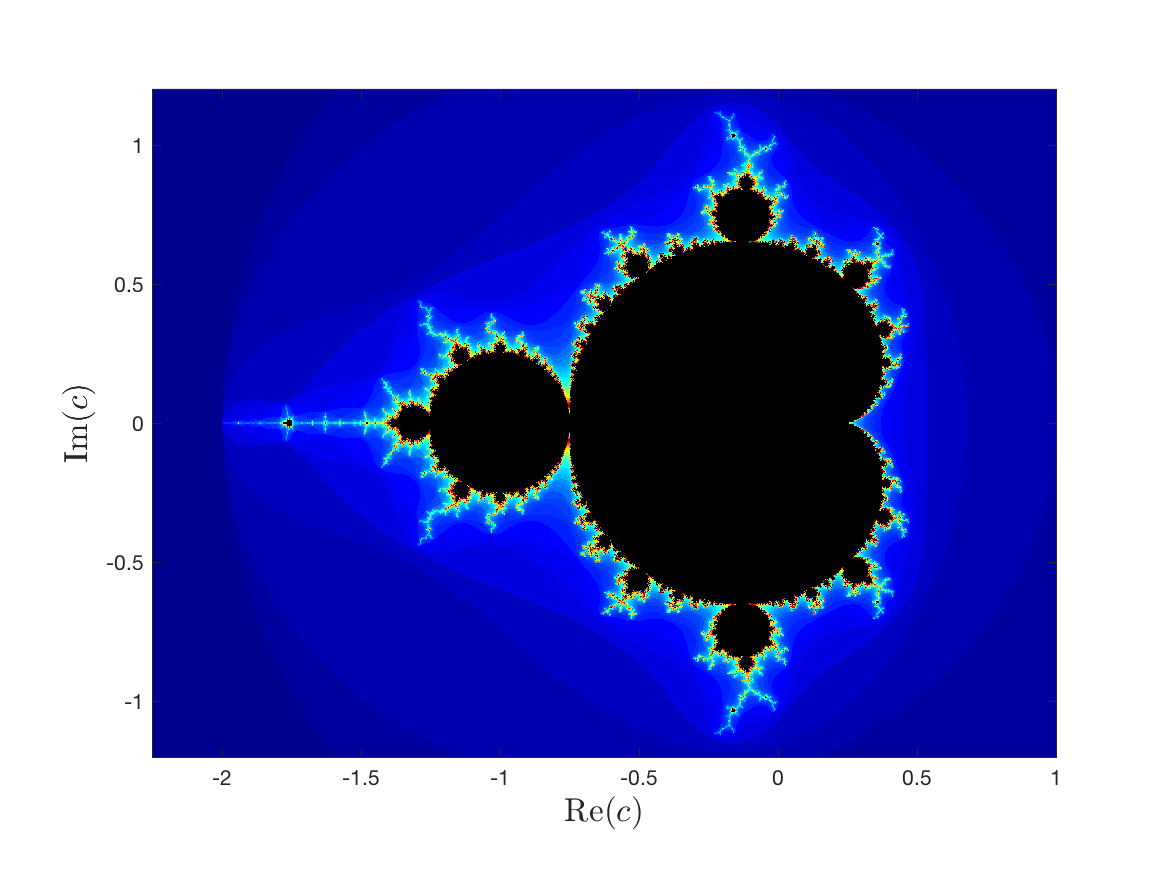
\includegraphics[width = 0.6\textwidth]{Images/mandelbrot} % enter the filename here
% 		\caption{This is a figure caption, note how it appears underneath the figure.} % enter the figure caption here
% 		\label{fig:figure label} % enter the figure label here (for cross referencing)
% 	\end{center}
% \end{figure}

% % ------------------------------------------------------------------------------
% % Table example
% % ------------------------------------------------------------------------------
% \begin{table}[H]
% 	\caption{This is a table caption, not how it appears above the table.}
% 	\label{tab:table label} % enter the table label here (for cross referencing)
% 	\begin{center}
% 		\begin{tabular}{lcr} % three columns aligned left, centre and right respectively
% 			\toprule % thick horizontal line at the top of the table
% 			first column & second column & third column \\
% 			\midrule % single horizontal line separating the column headings
% 			This & This & This \\
% 			column & column & column \\
% 			is left & is centrally & is right \\
% 			aligned & aligned & aligned \\
% 			\bottomrule % thick horizontal line at the bottom of the table
% 		\end{tabular}
% 	\end{center}
% \end{table}

% \subsection{Program code}

% % ------------------------------------------------------------------------------
% % Code listing example
% % ------------------------------------------------------------------------------
% \begin{lstlisting}[style=matlabcode,
%     caption = A MATLAB function to compute the first $n$ numbers of the Fibonacci series,
%     label = mat:fibonacci
%     ]
% function y = fibonacci(n)

% % This function calculates the first n terms in the Fibonacci series

% y(1) = 0;
% y(2) = 1;

% for i = 3 : n
%     y(i) = y(i-2) + y(i-1)
% end

% end
% \end{lstlisting}

% % ------------------------------------------------------------------------------
% % Referencing examples
% % ------------------------------------------------------------------------------
% \section{Referencing}
% References can be cited so that the author names(s) are a part of the sentence, e.g., \textcite{stroud:2013}, \textcite{harten:1983}

% Alternatively, references can be cited so that the author names appear in the brackets (for when the name of the author is not relevant to the sentence), e.g., \parencite{stroud:2013},  \parencite{harten:1983}.

% Cross referencing is easily done by using the label of the item you are referencing to (see source code for details).
% \begin{itemize}
% 	\item Chapter~\ref{cha:chapter label}
% 	\item Section~\ref{sec:section label}
% 	\item Equation~(\ref{eq:equation label})
% 	\item Table~\ref{tab:table label}
% 	\item Figure~\ref{fig:figure label}
% 	\item Page~\pageref{eq:equation label}
% \end{itemize}

% Above is an example of a bulleted list. You can also create numbered lists:
% \begin{enumerate}
% 	\item First list item
% 	\item Second list item
% 	\begin{enumerate}
% 		\item First sub list item
% 		\item Second sub list item
% 	\end{enumerate}
% 	\item Third list item
% \end{enumerate}
